\section{Loss Plot}

\begin{figure}[H]
  \centering
  \includegraphics[width=0.8\textwidth]{figures/loss-plot.pdf}
  \caption{Loss Plot}
  \label{fig:loss-plot}
\end{figure}

The loss decreases steadily over time as the model learns the alignments
between the source and target words.
We also see periodic spikes in the loss, which are likely caused by the
model learning specific translations that it had not encountered before,
and the loss eventually drops again as the model generalizes the 
learned translations to other examples.

% final loss values
\begin{small}
\begin{verbatim}
                                                 .
                                                 .
                                                 .
Epoch:  81 | Train loss: 0.012 | Val loss: 0.095 | Gen: ethay airway onditingcay isway orkingway
Epoch:  82 | Train loss: 0.006 | Val loss: 0.098 | Gen: ethay airway onditingcay isway orkingway
Epoch:  83 | Train loss: 0.005 | Val loss: 0.092 | Gen: ethay airway onditiningcay isway orkingway
Epoch:  84 | Train loss: 0.007 | Val loss: 0.150 | Gen: ethay airway onditiningcay isway orkingway
Epoch:  85 | Train loss: 0.021 | Val loss: 0.141 | Gen: ethay airway onditiningcay isway orkingway
Epoch:  86 | Train loss: 0.013 | Val loss: 0.081 | Gen: ethay airway onditiningcay isway orkingway
Epoch:  87 | Train loss: 0.006 | Val loss: 0.088 | Gen: ethay airway onditingcay isway orkingway
Epoch:  88 | Train loss: 0.004 | Val loss: 0.082 | Gen: ethay airway onditiningcay isway orkingway
Epoch:  89 | Train loss: 0.006 | Val loss: 0.091 | Gen: ethay airway onditingcay isway orkingway
Epoch:  90 | Train loss: 0.003 | Val loss: 0.082 | Gen: ethay airway onditiningcay isway orkingway
Epoch:  91 | Train loss: 0.003 | Val loss: 0.083 | Gen: ethay airway onditiningcay isway orkingway
Epoch:  92 | Train loss: 0.002 | Val loss: 0.086 | Gen: ethay airway onditiningcay isway orkingway
Epoch:  93 | Train loss: 0.002 | Val loss: 0.077 | Gen: ethay airway onditiningcay isway orkingway
Epoch:  94 | Train loss: 0.002 | Val loss: 0.104 | Gen: ethay airway onditiningcay isway orkingway
Epoch:  95 | Train loss: 0.009 | Val loss: 0.119 | Gen: ethay airway onditingcay isway orkingway
Epoch:  96 | Train loss: 0.028 | Val loss: 1.268 | Gen: ethay airway onditiondgway issway orkingway
Epoch:  97 | Train loss: 0.092 | Val loss: 0.256 | Gen: ethay airway onditingcay isway orkingway
Epoch:  98 | Train loss: 0.028 | Val loss: 0.112 | Gen: ethay airway onditioningcay isway orkingway
Epoch:  99 | Train loss: 0.013 | Val loss: 0.110 | Gen: ethay airway onditioningcay isway orkingway
Epoch: 100 | Train loss: 0.005 | Val loss: 0.101 | Gen: ethay airway onditioningcay isway orkingway
source:         the air conditioning is working
translated:     ethay airway onditioningcay isway orkingway
\end{verbatim}
\end{small}

\newpage
\section{Attention Visualizations}

\begin{enumarabic}
  \item \verb|cake| $\mapsto$ \verb|akecay| \\
    The transformer translates \verb|cake| to \verb|akecay|, which is the correct translation.
    Looking at the attention visualizations, the model's alignment of the source
    and target words gets more accurate and confident in the second and third layers.

    \begin{figure}[H]
      %  minipages
      \centering
      \begin{minipage}[b]{0.33\textwidth}
        \centering
        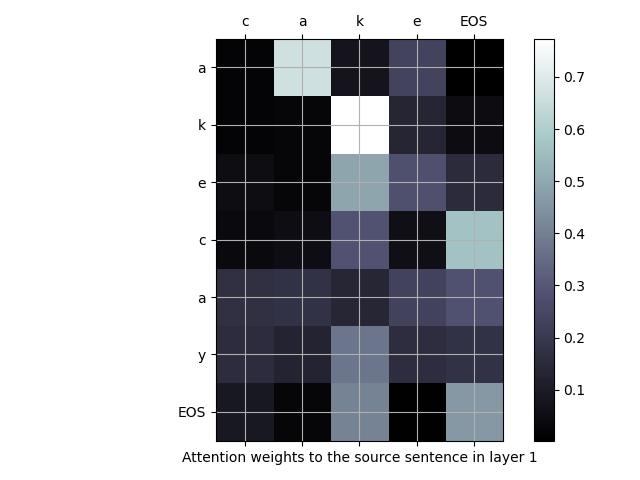
\includegraphics[width=\textwidth]{figures/cake-0.png}
        \caption{Layer 1}
        \label{fig:cake-0}
      \end{minipage}
      \hfill
      \begin{minipage}[b]{0.33\textwidth}
        \centering
        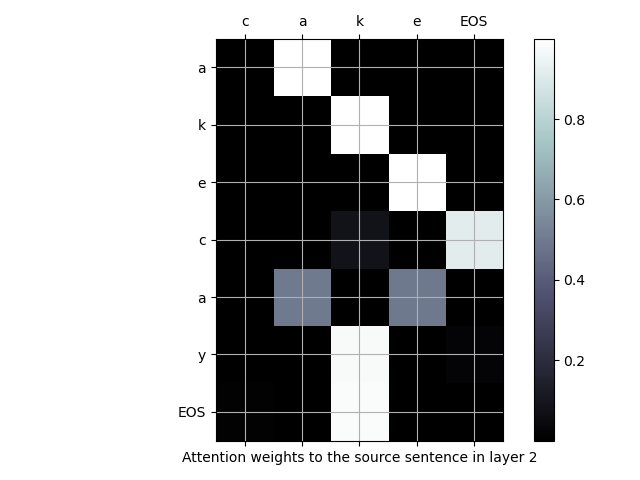
\includegraphics[width=\textwidth]{figures/cake-1.png}
        \caption{Layer 2}
        \label{fig:cake-1}
      \end{minipage}
      \begin{minipage}[b]{0.33\textwidth}
        \centering
        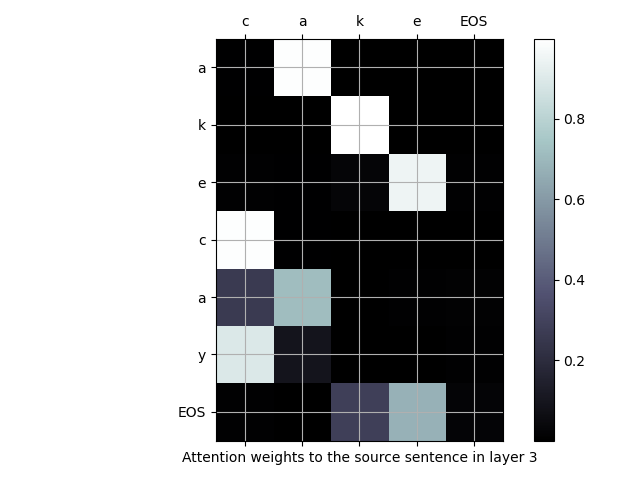
\includegraphics[width=\textwidth]{figures/cake-2.png}
        \caption{Layer 3}
        \label{fig:cake-2}
      \end{minipage}
    \end{figure}

  \item \verb|drink| $\mapsto$ \verb|inkdray| \\
    The transformer translates \verb|drink| to \verb|inkdray|, which is the correct translation.
    The alignment of the source and target words is also accurate and most confident
    in the third layer.

    \begin{figure}[H]
      %  minipages
      \centering
      \begin{minipage}[b]{0.33\textwidth}
        \centering
        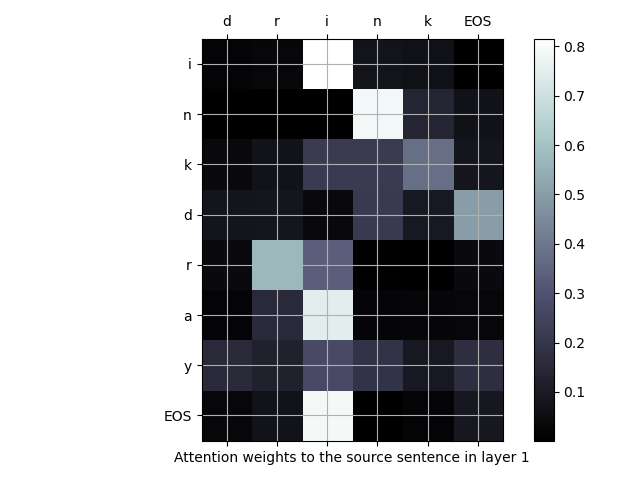
\includegraphics[width=\textwidth]{figures/drink-0.png}
        \caption{Layer 1}
        \label{fig:drink-0}
      \end{minipage}
      \hfill
      \begin{minipage}[b]{0.33\textwidth}
        \centering
        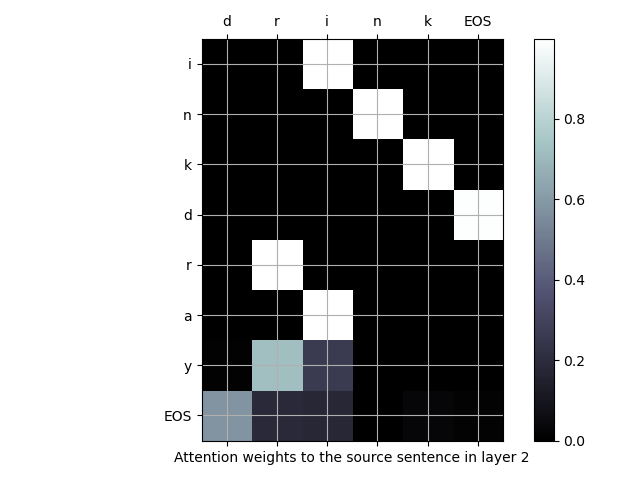
\includegraphics[width=\textwidth]{figures/drink-1.png}
        \caption{Layer 2}
        \label{fig:drink-1}
      \end{minipage}
      \begin{minipage}[b]{0.33\textwidth}
        \centering
        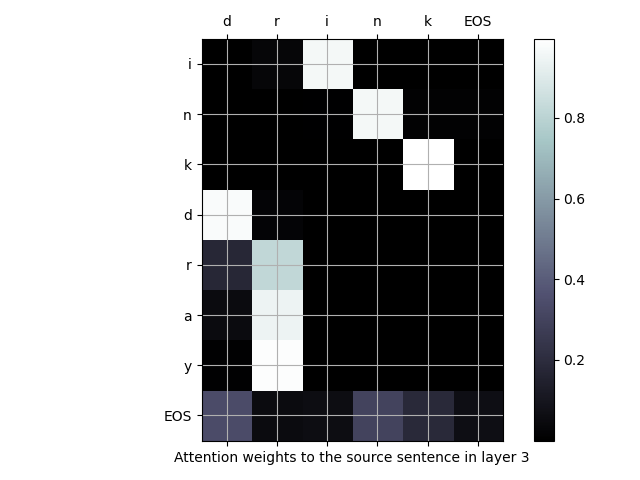
\includegraphics[width=\textwidth]{figures/drink-2.png}
        \caption{Layer 3}
        \label{fig:drink-2}
      \end{minipage}
    \end{figure}

  \item \verb|aardvark| $\mapsto$ \verb|awarkway| \\
    The transformer translates this word incorrectly.
    Instead of \verb|awarkway|, the correct translation is \verb|aardvarkway|.
    Looking at the attention visualizations, the model's alignment of the source
    and target words is noisy in the first layer and gets more confident in subsequent
    layers. However, the alignment is not accurate aside from the first two letters!
    This suggests that the model is not able to align the source and target words
    correctly, which is likely the cause of the error in translation.
    
    \begin{figure}[H]
      %  minipages
      \centering
      \begin{minipage}[b]{0.33\textwidth}
        \centering
        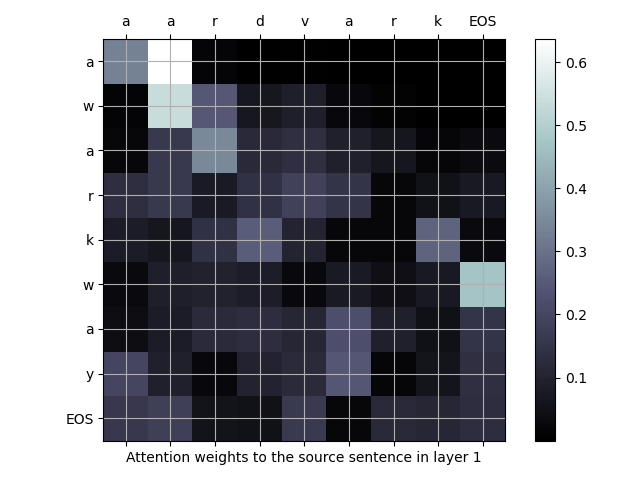
\includegraphics[width=\textwidth]{figures/aardvark-0.png}
        \caption{Layer 1}
        \label{fig:aardvark-0}
      \end{minipage}
      \hfill
      \begin{minipage}[b]{0.33\textwidth}
        \centering
        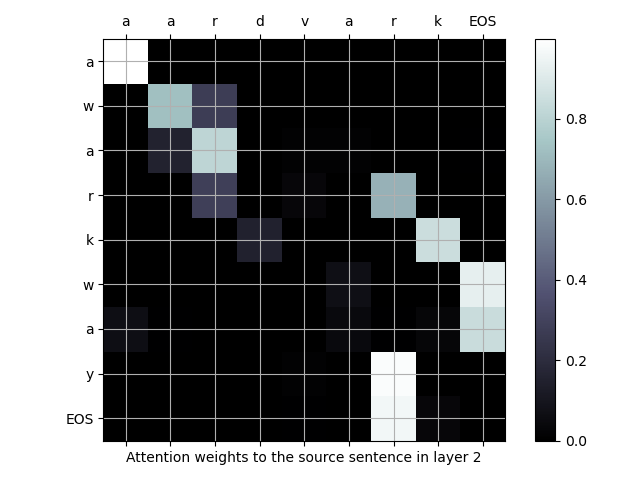
\includegraphics[width=\textwidth]{figures/aardvark-1.png}
        \caption{Layer 2}
        \label{fig:aardvark-1}
      \end{minipage}
      \begin{minipage}[b]{0.33\textwidth}
        \centering
        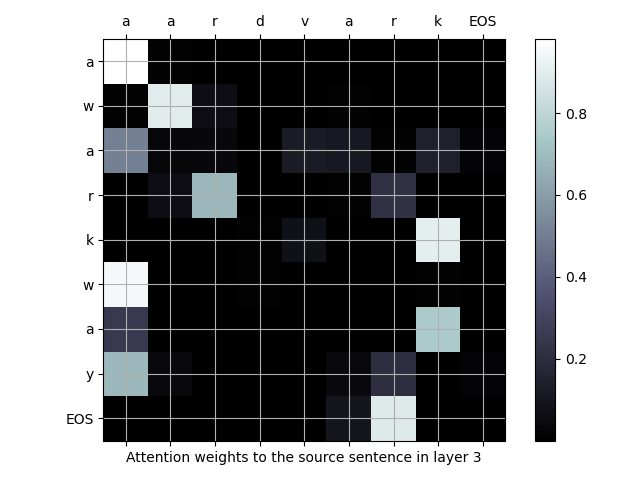
\includegraphics[width=\textwidth]{figures/aardvark-2.png}
        \caption{Layer 3}
        \label{fig:aardvark-2}
      \end{minipage}
    \end{figure}

  \newpage
  \item \verb|well-mannered| $\mapsto$ \verb|ellway-anneredmay| \\
    This is a particularly interesting example since it involves a hyphenated word,
    and the transformer translates each part of the hyphenated word separately,
    correctly, and joins them with a hyphen in the correct order.
    Looking at the attention plots, we also see the model's alignment
    being noisy in the first layer, but more accurate and confident in the second,
    and eventually most-accurate in the third layer.
    \begin{figure}[H]
      %  minipages
      \centering
      \begin{minipage}[b]{0.33\textwidth}
        \centering
        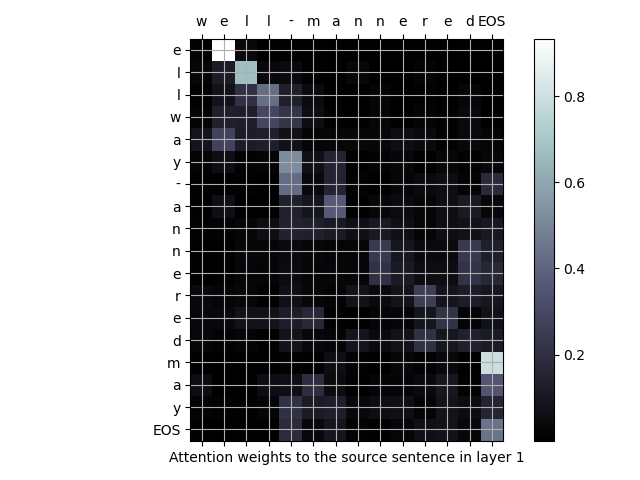
\includegraphics[width=\textwidth]{figures/well-mannered-0.png}
        \caption{Layer 1}
        \label{fig:well-mannered-0}
      \end{minipage}
      \hfill
      \begin{minipage}[b]{0.33\textwidth}
        \centering
        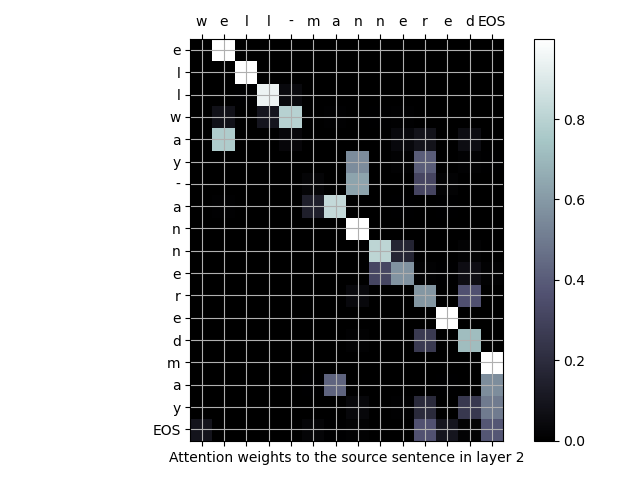
\includegraphics[width=\textwidth]{figures/well-mannered-1.png}
        \caption{Layer 2}
        \label{fig:well-mannered-1}
      \end{minipage}
      \begin{minipage}[b]{0.33\textwidth}
        \centering
        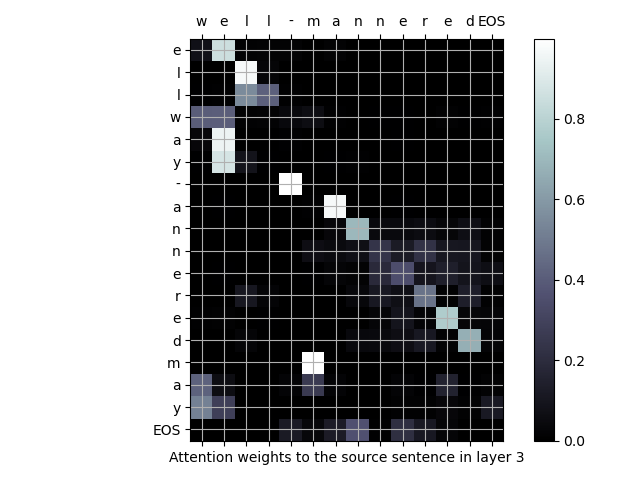
\includegraphics[width=\textwidth]{figures/well-mannered-2.png}
        \caption{Layer 3}
        \label{fig:well-mannered-2}
      \end{minipage}
    \end{figure}

  \item \verb|amittai| $\mapsto$ \verb|amittaiway| \\
    This is not a proper English word (it's actually my first name). \\
    The transformer translates it correctly as \verb|amittaiway|. \\
    Looking at the attention visualizations, we can see that the model
    is able to align the source and target words correctly,
    with the attention weights being more confident in the second and the third layer.
    \begin{figure}[H]
      %  minipages
      \centering
      \begin{minipage}[b]{0.33\textwidth}
        \centering
        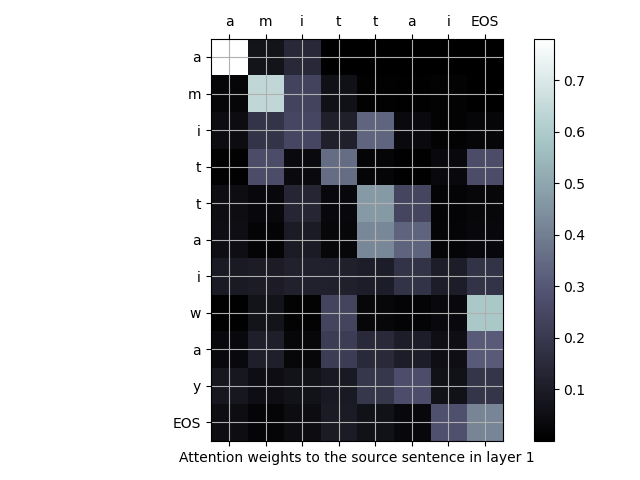
\includegraphics[width=\textwidth]{figures/amittai-0.png}
        \caption{Layer 1}
        \label{fig:amittai-0}
      \end{minipage}
      \hfill
      \begin{minipage}[b]{0.33\textwidth}
        \centering
        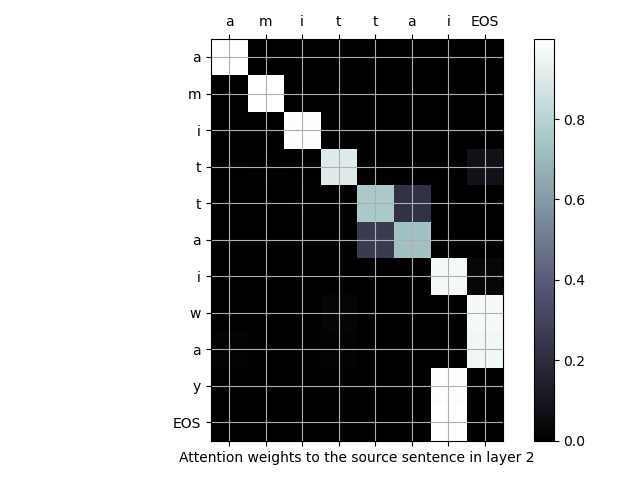
\includegraphics[width=\textwidth]{figures/amittai-1.png}
        \caption{Layer 2}
        \label{fig:amittai-1}
      \end{minipage}
      \begin{minipage}[b]{0.33\textwidth}
        \centering
        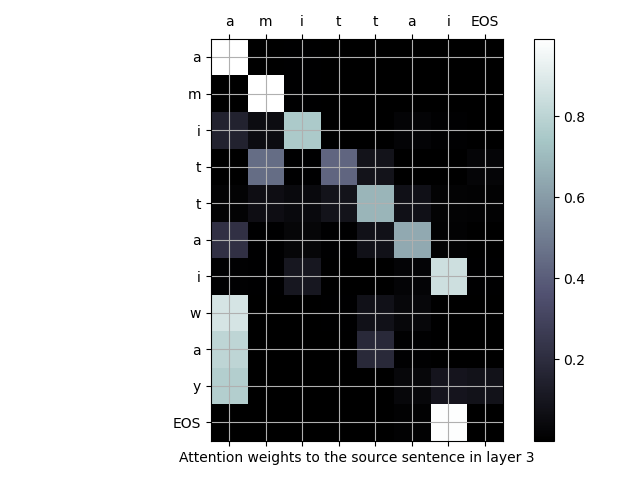
\includegraphics[width=\textwidth]{figures/amittai-2.png}
        \caption{Layer 3}
        \label{fig:amittai-2}
      \end{minipage}
    \end{figure}

  \item \verb|siavava| $\mapsto$ \verb|iavavassay| \\
    The transformer was close to getting the correct translation,
    but failed by translating to \verb|iavavassay| instead of \verb|iavavasay|
    (two \verb|s| instead of one).
    Looking at the attention visualizations, the model's attention weights
    in the second layer, and most confident in the third layer.
    We also see some noise in the third layer where the \verb|a|
    in the result is, which is likely caused by the error in producing two \verb|s|'s.

    \begin{figure}[H]
      %  minipages
      \centering
      \begin{minipage}[b]{0.33\textwidth}
        \centering
        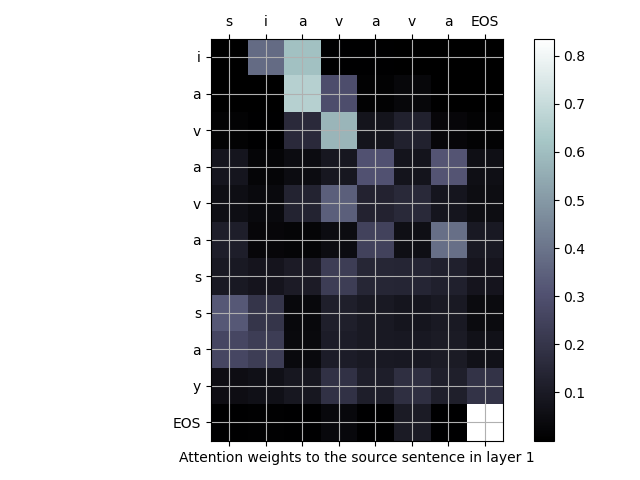
\includegraphics[width=\textwidth]{figures/siavava-0.png}
        \caption{Layer 1}
        \label{fig:siavava-0}
      \end{minipage}
      \hfill
      \begin{minipage}[b]{0.33\textwidth}
        \centering
        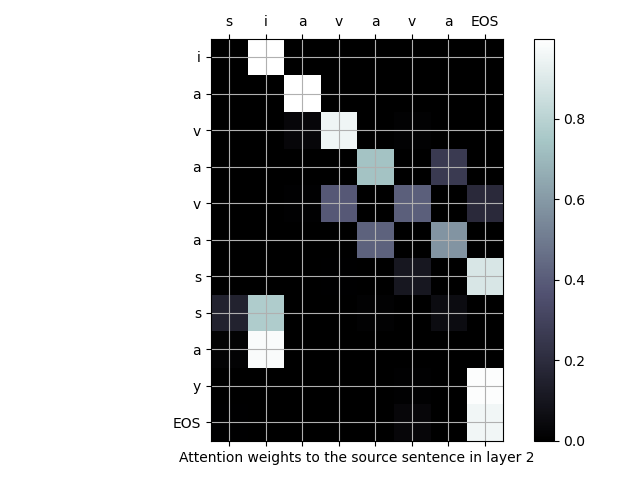
\includegraphics[width=\textwidth]{figures/siavava-1.png}
        \caption{Layer 2}
        \label{fig:siavava-1}
      \end{minipage}
      \begin{minipage}[b]{0.33\textwidth}
        \centering
        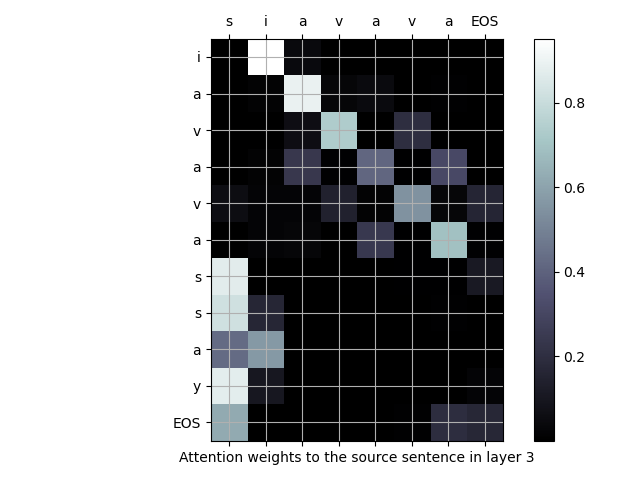
\includegraphics[width=\textwidth]{figures/siavava-2.png}
        \caption{Layer 3}
        \label{fig:siavava-2}
      \end{minipage}
    \end{figure}

  \item \verb|wekesa| $\mapsto$ \verb|ekesay| \\
    \verb|wekesa| is my surname.
    The transformer translates it to \verb|ekesay|, instead of the correct \verb|ekesaway|. \\
    Looking at the attention visualizations, the model
    develops an accurate alignment between the source and target words,
    but fails to produce the correct translation, likely because of the specific
    nature of the word.

    \begin{figure}[H]
      %  minipages
      \centering
      \begin{minipage}[b]{0.33\textwidth}
        \centering
        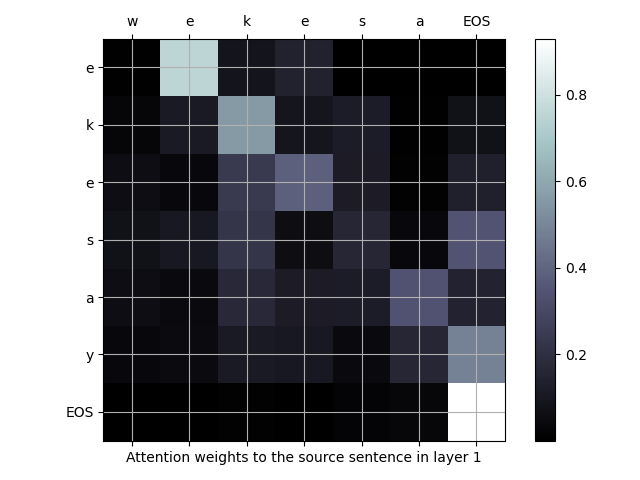
\includegraphics[width=\textwidth]{figures/wekesa-0.png}
        \caption{Layer 1}
        \label{fig:wekesa-0}
      \end{minipage}
      \hfill
      \begin{minipage}[b]{0.33\textwidth}
        \centering
        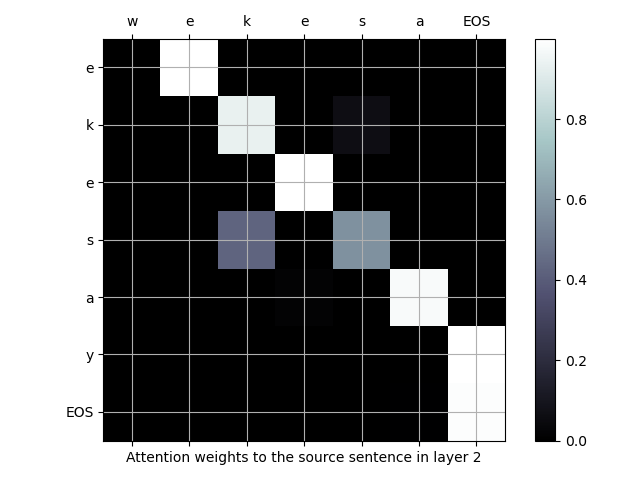
\includegraphics[width=\textwidth]{figures/wekesa-1.png}
        \caption{Layer 2}
        \label{fig:wekesa-1}
      \end{minipage}
      \begin{minipage}[b]{0.33\textwidth}
        \centering
        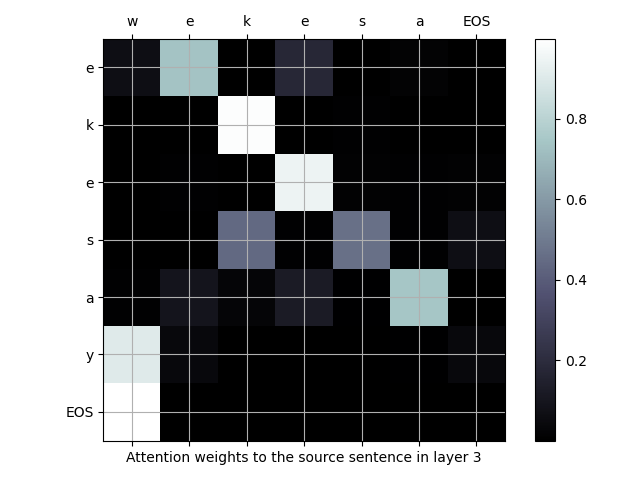
\includegraphics[width=\textwidth]{figures/wekesa-2.png}
        \caption{Layer 3}
        \label{fig:wekesa-2}
      \end{minipage}
    \end{figure}
    
\end{enumarabic}





